\chapter{Interactions intermoléculaires et solvants}\label{ch:b1:intermolecular-forces-solvents}

Un gecko court sur une vitre et s'y suspend par un seul doigt~: ni
colle, ni ventouse, rien que l'attraction entre les molécules de ses
pelotes digitales et celles du verre. L'eau, molécule plus légère que le
dioxyde de carbone, bout à \qty{100}{\celsius}, alors que le dioxyde de
carbone est un gaz à température ambiante. L'huile flotte sur le
vinaigre sans jamais s'y mélanger~; le sel de cuisine se dissout dans
l'eau et pas dans l'essence. Tous ces faits sont décidés non par les
liaisons à l'intérieur des molécules, mais par les forces, bien plus
faibles, qui s'exercent entre elles. Ce chapitre classe ces forces,
mesure leurs effets sur les températures d'ébullition et s'en sert pour
choisir un solvant.

% ledger: bp:H2O (the hook's 100 degC)

\begin{recall}
Le livre 1 (année 11) a introduit les \omterm{def:b1:intermolecular-forces-solvents:vdw}{interactions de van der Waals} et
les \omterm{def:b1:intermolecular-forces-solvents:hbond}{liaisons hydrogène}, et expliqué que les solides ioniques se
dissolvent par dissociation et \omterm{def:b1:intermolecular-forces-solvents:dissolution}{solvatation}. Les \omterm{def:b1:lewis-resonance-vsepr:dipole}{moments dipolaires} ont
été définis à la \cref{def:b1:lewis-resonance-vsepr:dipole} et la
\omterm{def:b1:periodicity:polarisability}{polarisabilité} à la \cref{def:b1:periodicity:polarisability}. On utilise
la loi de Coulomb, vue en physique~: deux charges $q_1$ et $q_2$ à la
distance $r$ dans le vide s'attirent ou se repoussent avec une force de
norme $|q_1q_2|/(4\pi
\varepsilon_0 r^2)$.
\end{recall}

\begin{omfigure}
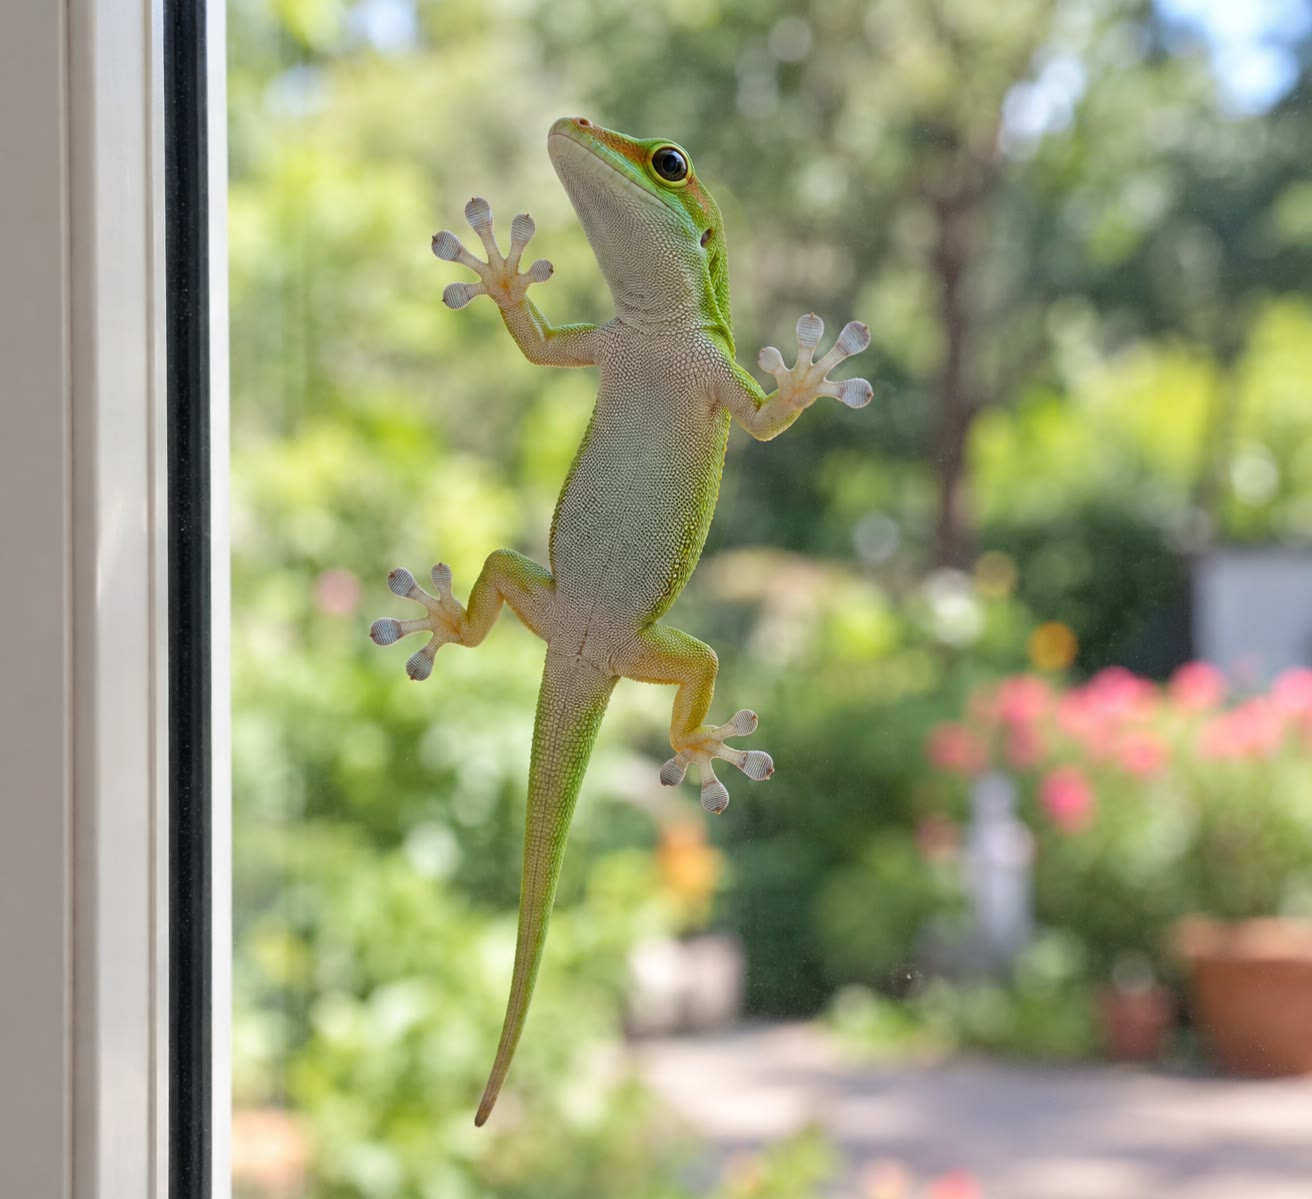
\includegraphics[width=0.52\linewidth]{images/book2/ai/b1-04-gecko.jpg}

{\small Un gecko sur une vitre. Les millions de poils fins de ses
pelotes digitales s'approchent tant du verre que la faible attraction
entre leurs molécules et celles du verre finit par dépasser son poids.}
\end{omfigure}

\section{Interactions de van der Waals}

\begin{definition}[Interactions de van der Waals]\label{def:b1:intermolecular-forces-solvents:vdw}
Les \emph{interactions de van der Waals}\index{interaction de van der Waals}
sont les attractions entre molécules neutres qui proviennent de
l'interaction de leurs dipôles. On en distingue trois sortes~:
\begin{itemize}
  \item l'\emph{interaction de Keesom}\index{interaction de Keesom} (ou
        interaction d'orientation) entre deux dipôles permanents, qui
        tendent à s'aligner tête-bêche~;
  \item l'\emph{interaction de Debye}\index{interaction de Debye} (ou
        interaction d'induction) entre un dipôle permanent et le dipôle
        qu'il induit dans un voisin polarisable~;
  \item l'\emph{interaction de London}\index{interaction de London} (ou
        interaction de dispersion) entre les dipôles instantanés que les
        fluctuations des nuages électroniques créent dans deux atomes ou
        molécules quelconques, polaires ou non, et qui s'induisent
        mutuellement.
\end{itemize}
\end{definition}

\begin{omfigure}
\begin{tikzpicture}[font=\small, >={Stealth},
    mol/.style={draw=black!60, fill=#1, ellipse, minimum width=1.5cm, minimum height=0.8cm}]
  % Keesom
  \node[mol=omDef!20] (a) at (0,0) {}; \node[mol=omDef!20] (b) at (1.7,0) {};
  \node at (-0.45,0) {$\delta^-$}; \node at (0.45,0) {$\delta^+$};
  \node at (1.25,0) {$\delta^-$}; \node at (2.15,0) {$\delta^+$};
  \node[below, align=center] at (0.85,-0.65) {Keesom~:\\deux dipôles permanents};
  % Debye
  \begin{scope}[xshift=4.6cm]
    \node[mol=omDef!20] at (0,0) {}; \node[mol=black!5, dashed] at (1.7,0) {};
    \node at (-0.45,0) {$\delta^-$}; \node at (0.45,0) {$\delta^+$};
    \node[omProp] at (1.25,0) {$\delta^-$}; \node[omProp] at (2.15,0) {$\delta^+$};
    \node[below, align=center] at (0.85,-0.65) {Debye~:\\permanent et induit};
  \end{scope}
  % London
  \begin{scope}[xshift=9.2cm]
    \node[mol=black!5, dashed] at (0,0) {}; \node[mol=black!5, dashed] at (1.7,0) {};
    \node[omProp] at (-0.45,0) {$\delta^-$}; \node[omProp] at (0.45,0) {$\delta^+$};
    \node[omProp] at (1.25,0) {$\delta^-$}; \node[omProp] at (2.15,0) {$\delta^+$};
    \node[below, align=center] at (0.85,-0.65) {London~:\\deux dipôles instantanés};
  \end{scope}
\end{tikzpicture}

{\small Les trois \omterm{def:b1:intermolecular-forces-solvents:vdw}{interactions de van der Waals}. Les charges partielles
noires sont permanentes (\omterm{def:b1:lewis-resonance-vsepr:dipole}{molécules polaires})~; les orange sont induites
ou instantanées. Dans chaque cas, les charges en regard sont opposées~:
les molécules s'attirent.}
\end{omfigure}

\begin{proposition}[Intensité et portée]\label{prop:b1:intermolecular-forces-solvents:distance-law}
Pour deux molécules à la distance $r$, chacune des trois énergies de van
der Waals varie comme $-1/r^6$~: l'attraction ne se fait sentir qu'entre
voisins. Ces énergies sont de l'ordre de quelques kilojoules par mole,
environ cent fois moins qu'une \omterm{def:b1:lewis-resonance-vsepr:lewis}{liaison covalente}. Le terme de London
croît avec les \omterm{def:b1:periodicity:polarisability}{polarisabilités} des deux partenaires~; il existe entre
toutes les molécules et c'est en général le plus grand des trois, sauf
pour les petites molécules très polaires.
\end{proposition}
\admitted

\begin{example}[Gaz nobles et halogènes]\label{ex:b1:intermolecular-forces-solvents:noble}
Les atomes d'un gaz noble ne s'attirent que par des forces de London,
qui croissent avec le nombre d'électrons~: l'hélium bout à
\qty{-268.9}{\celsius}, le néon à \qty{-246.1}{\celsius}, l'argon à
\qty{-185.9}{\celsius}, le krypton à \qty{-153.4}{\celsius}, le xénon à
\qty{-108.1}{\celsius}. De même, à température ambiante, le difluor et le
dichlore sont gazeux, le dibrome liquide (il bout à \qty{58.8}{\celsius})
et le diiode solide.
% ledger: bp:He, bp:Ne, bp:Ar, bp:Kr, bp:Xe, bp:F2, bp:Cl2, bp:Br2, bp:I2
\end{example}

\begin{omfigure}
\begin{tikzpicture}
\begin{axis}[
  width=0.62\linewidth, height=5.4cm,
  xmin=0.5, xmax=10.5, ymin=-180, ymax=200,
  axis x line=bottom, axis y line=left,
  xlabel={nombre d'atomes de carbone $n$}, ylabel={température d'ébullition (\unit{\celsius})},
  xtick={1,2,3,4,5,6,7,8,9,10}, ytick={-150,-100,-50,0,50,100,150},
  tick label style={font=\small}, label style={font=\small}]
\addplot[omDef, thick, mark=*, mark size=1.5pt] table[x=n, y=bp_C] {figdata/out/bachelor-1-hydride-boiling-points-alkanes.dat};
\end{axis}
\end{tikzpicture}

{\small Températures d'ébullition des alcanes linéaires \ce{C_nH_{2n+2}},
du méthane au décane. Chaque \ce{CH2} ajouté apporte des électrons et de
la surface de contact, donc de l'attraction de London~; l'incrément
diminue lentement, d'environ \qty{75}{\celsius} au début à
\qty{25}{\celsius} au décane.}
\end{omfigure}

\section{La liaison hydrogène}

\begin{definition}[Liaison hydrogène]\label{def:b1:intermolecular-forces-solvents:hbond}
Une \emph{liaison hydrogène}\index{liaison hydrogene@liaison hydrogène} est une attraction
$\ce{X-H}\cdots\ce{Y}$ entre un atome d'hydrogène lié à un atome X petit
et très électronégatif (\ce{N}, \ce{O} ou \ce{F}) et un \omterm{def:b1:lewis-resonance-vsepr:lewis}{doublet non liant}
d'un autre atome électronégatif Y. La molécule qui porte \ce{X-H} est le
donneur de liaison hydrogène, celle qui porte Y l'accepteur. Son
énergie, de 10 à \qty{40}{kJ/mol}, est intermédiaire entre celles des
\omterm{def:b1:intermolecular-forces-solvents:vdw}{interactions de van der Waals} et des \omterm{def:b1:lewis-resonance-vsepr:lewis}{liaisons covalentes}~; les trois
atomes \ce{X}, \ce{H}, \ce{Y} sont presque alignés.
\end{definition}

\begin{remark}[Pourquoi N, O et F]\label{rem:b1:intermolecular-forces-solvents:why}
Un atome X fortement électronégatif laisse à l'hydrogène une forte
charge partielle positive~; l'hydrogène, qui n'a pas d'électrons
internes, est minuscule, si bien que le \omterm{def:b1:lewis-resonance-vsepr:lewis}{doublet non liant} de Y peut s'en
approcher de très près. Les deux conditions sont nécessaires~: les
liaisons \ce{C-H} ne sont pas assez polarisées, et les liaisons \ce{S-H}
ou \ce{Cl-H} mettent en jeu des atomes trop gros et trop peu
électronégatifs pour former des \omterm{def:b1:intermolecular-forces-solvents:hbond}{liaisons hydrogène} fortes.
\end{remark}

\begin{omfigure}
\begin{tikzpicture}[font=\small]
  % water network
  \foreach \n/\x/\y/\a in {1/0/0/0, 2/2.2/0.9/200, 3/0.2/-2.0/60, 4/-2.1/0.6/-30} {
    \begin{scope}[shift={(\x,\y)}, rotate=\a]
      \node[aO] (o\n) at (0,0) {};
      \node[aH] (h\n a) at (0.78,0.3) {};
      \node[aH] (h\n b) at (-0.2,-0.82) {};
      \begin{scope}[on background layer]
        \draw[bond] (o\n.center) -- (h\n a.center); \draw[bond] (o\n.center) -- (h\n b.center);
      \end{scope}
    \end{scope}
  }
  \draw[omThm, thick, densely dotted] (h1a) -- (o2);
  \draw[omThm, thick, densely dotted] (h1b) -- (o3);
  \draw[omThm, thick, densely dotted] (h4a) -- (o1);
  \node[below] at (0,-2.9) {eau~: chaque molécule peut en donner deux et en accepter deux};
  % carboxylic acid dimer
  \begin{scope}[xshift=5.6cm, yshift=-0.6cm]
    \node (r1) at (-0.9,0) {R}; \node (c1) at (0,0) {C};
    \node (o1) at (0.6,0.85) {O}; \node (o2) at (0.6,-0.85) {O}; \node (h2) at (1.45,-0.85) {H};
    \node (c2) at (3.3,0) {C}; \node (r2) at (4.2,0) {R};
    \node (o3) at (2.7,0.85) {O}; \node (o4) at (2.7,-0.85) {O}; \node (h3) at (1.85,0.85) {H};
    \draw (r1) -- (c1) -- (o2) -- (h2) (c2) -- (r2) (c2) -- (o3) -- (h3);
    \draw[double, double distance=1.6pt] (c1) -- (o1); \draw[double, double distance=1.6pt] (c2) -- (o4);
    \draw[omThm, thick, densely dotted] (h2) -- (o4) (h3) -- (o1);
    \node[below] at (1.65,-2.3) {un dimère d'acide carboxylique};
  \end{scope}
\end{tikzpicture}

{\small \omterm{def:b1:intermolecular-forces-solvents:hbond}{Liaisons hydrogène} (pointillés rouges). Dans l'eau liquide, chaque
molécule participe à quatre d'entre elles au plus~; les acides
carboxyliques s'associent en dimères cycliques tenus par deux \omterm{def:b1:intermolecular-forces-solvents:hbond}{liaisons
hydrogène}.}
\end{omfigure}

\begin{proposition}[Les liaisons hydrogène élèvent les températures d'ébullition]\label{prop:b1:intermolecular-forces-solvents:hbond-bp}
Parmi les hydrures des \omterm{def:b1:periodicity:table}{groupes} 15, 16 et 17, la température d'ébullition
augmente de la \omterm{def:b1:periodicity:table}{période} 3 à la \omterm{def:b1:periodicity:table}{période} 5, en suivant l'\omterm{def:b1:intermolecular-forces-solvents:vdw}{interaction de
London}~; les hydrures de la \omterm{def:b1:periodicity:table}{période} 2, \ce{NH3}, \ce{H2O} et \ce{HF}, qui
forment des \omterm{def:b1:intermolecular-forces-solvents:hbond}{liaisons hydrogène}, bouillent bien au-dessus de
l'extrapolation de cette tendance. Les hydrures du \omterm{def:b1:periodicity:table}{groupe} 14 (\ce{CH4},
\ce{SiH4}, \ce{GeH4}) ne forment pas de \omterm{def:b1:intermolecular-forces-solvents:hbond}{liaisons hydrogène} et suivent la
tendance.
\end{proposition}

\begin{omfigure}
\begin{tikzpicture}
\begin{axis}[
  width=0.82\linewidth, height=6.6cm,
  xmin=1.5, xmax=5.6, ymin=-180, ymax=120,
  axis x line=bottom, axis y line=left,
  xlabel={période}, ylabel={température d'ébullition (\unit{\celsius})},
  xtick={2,3,4,5}, ytick={-150,-100,-50,0,50,100},
  tick label style={font=\small}, label style={font=\small},
  clip=false]
\addplot[black!60, thick, mark=square*, mark size=1.6pt] table[x=period, y=bp_C] {figdata/out/bachelor-1-hydride-boiling-points-g14.dat};
\addplot[omDef, thick, mark=*, mark size=1.6pt] table[x=period, y=bp_C] {figdata/out/bachelor-1-hydride-boiling-points-g15.dat};
\addplot[omThm, thick, mark=*, mark size=1.6pt] table[x=period, y=bp_C] {figdata/out/bachelor-1-hydride-boiling-points-g16.dat};
\addplot[omMeth, thick, mark=triangle*, mark size=2pt] table[x=period, y=bp_C] {figdata/out/bachelor-1-hydride-boiling-points-g17.dat};
\addplot[omThm, dashed] coordinates {(2,-79.3) (3,-60.3)};
\node[font=\small, anchor=west] at (axis cs:2.05,100) {\ce{H2O}};
\node[font=\small, anchor=west] at (axis cs:2.05,19.6) {\ce{HF}};
\node[font=\small, anchor=west] at (axis cs:2.05,-30) {\ce{NH3}};
\node[font=\small, anchor=east] at (axis cs:1.96,-162) {\ce{CH4}};
\node[font=\small, anchor=west] at (axis cs:4.05,-41.3) {\ce{H2Se}};
\node[font=\small, anchor=west] at (axis cs:5.05,-18.4) {\ce{SbH3}};
\node[font=\small, anchor=west] at (axis cs:5.05,-35.1) {\ce{HI}};
\node[font=\small, anchor=west] at (axis cs:4.05,-88.1) {\ce{GeH4}};
\node[font=\small, omThm, anchor=north west] at (axis cs:2.05,-85) {extrapolation};
\end{axis}
\end{tikzpicture}

{\small Températures d'ébullition des hydrures des \omterm{def:b1:periodicity:table}{groupes} 14 (carrés
gris), 15 (en bleu), 16 (en rouge) et 17 (en vert). L'eau bouillirait
vers \qty{-79}{\celsius} si elle suivait ses analogues plus lourds
(tirets)~; ses \omterm{def:b1:intermolecular-forces-solvents:hbond}{liaisons hydrogène} l'élèvent d'environ \qty{180}{\celsius}.}
% ledger: bp:CH4, bp:SiH4, bp:GeH4, bp:NH3, bp:PH3, bp:AsH3, bp:SbH3,
% bp:H2O, bp:H2S, bp:H2Se, bp:HF, bp:HCl, bp:HBr, bp:HI
\end{omfigure}

\begin{example}[L'éthanol et son isomère]\label{ex:b1:intermolecular-forces-solvents:isomers}
L'éthanol, \ce{CH3CH2OH}, et le méthoxyméthane, \ce{CH3OCH3}, ont la même
formule \ce{C2H6O} et presque les mêmes \omterm{def:b1:intermolecular-forces-solvents:vdw}{interactions de London}.
L'éthanol, dont le groupe \ce{O-H} est à la fois donneur et accepteur,
bout à \qty{78.4}{\celsius}~; le méthoxyméthane, qui ne peut
qu'accepter, bout à \qty{-25.0}{\celsius}.
% ledger: bp:C2H5OH, bp:CH3OCH3
\end{example}

\section{Solvants}

\begin{definition}[Permittivité relative]\label{def:b1:intermolecular-forces-solvents:permittivity}
Dans un milieu, la force de Coulomb entre deux charges est divisée par
un nombre $\varepsilon_r \ge 1$, la \emph{permittivité relative}\index{permittivite relative@permittivité relative}
(ou constante diélectrique) du milieu~:
\[
  F = \frac{|q_1 q_2|}{4\pi\varepsilon_0\varepsilon_r r^2} .
\]
Elle est grande pour les liquides de \omterm{def:b1:lewis-resonance-vsepr:dipole}{molécules polaires}, qui s'orientent
autour des charges et les écrantent~: \num{78.4} pour l'eau à
\qty{25}{\celsius}, \num{1.89} pour l'hexane à \qty{20}{\celsius}.
% ledger: epsr:H2O, epsr:C6H14
\end{definition}

\begin{definition}[Solvants polaires, protiques et aprotiques]\label{def:b1:intermolecular-forces-solvents:solvent-classes}
Un \emph{solvant polaire}\index{solvant polaire} est formé de molécules
de fort \omterm{def:b1:lewis-resonance-vsepr:dipole}{moment dipolaire} et possède une grande \omterm{def:b1:intermolecular-forces-solvents:permittivity}{permittivité relative}
(supérieure à 15 environ)~; un solvant apolaire en a une faible. Un
\emph{solvant protique}\index{solvant protique} a des molécules qui
portent des atomes d'hydrogène capables de former des \omterm{def:b1:intermolecular-forces-solvents:hbond}{liaisons hydrogène}
(\ce{O-H} ou \ce{N-H})~; un \emph{solvant
aprotique}\index{solvant aprotique} n'en a pas.
\end{definition}

\begin{center}
\small
\begin{tabular}{lccll}
\hline
solvant & $\varepsilon_r$ & $\mu$ (D) & polarité & proticité \\
\hline
eau & 78.4 & 1.86 & polaire & protique \\
méthanol & 32.6 & 1.67 & polaire & protique \\
éthanol & 24.3 & 1.52 & polaire & protique \\
acétonitrile, \ce{CH3CN} & 37.5 & 3.92 & polaire & aprotique \\
propanone (acétone) & 20.7 & 2.88 & polaire & aprotique \\
dichlorométhane & 9.08 & 1.62 & peu polaire & aprotique \\
éthanoate d'éthyle & 6.02 & 1.78 & peu polaire & aprotique \\
éthoxyéthane & 4.34 & 1.15 & peu polaire & aprotique \\
benzène & 2.28 & 0 & apolaire & aprotique \\
hexane & 1.89 & 0 & apolaire & aprotique \\
\hline
\end{tabular}
\end{center}
% ledger: epsr:H2O, epsr:CH3OH, epsr:C2H5OH, epsr:CH3CN, epsr:CH3COCH3,
% epsr:CH2Cl2, epsr:EtOAc, epsr:Et2O, epsr:C6H6, epsr:C6H14, dip:H2O,
% dip:CH3OH, dip:C2H5OH, dip:CH3CN, dip:CH3COCH3, dip:CH2Cl2, dip:EtOAc,
% dip:Et2O, dip:C6H6 (relative permittivities at 20 or 25 degC; dipole
% moments of the gas-phase molecules; hexane has no dipole by symmetry)

\begin{definition}[Solvatation, pouvoir ionisant et pouvoir dissociant]\label{def:b1:intermolecular-forces-solvents:dissolution}
La \emph{solvatation}\index{solvatation} d'une particule de soluté est
son enrobage par des molécules de solvant orientées et liées à elle par
des interactions intermoléculaires (on parle d'hydratation dans l'eau).
Le \emph{pouvoir
ionisant}\index{pouvoir ionisant} d'un solvant est sa capacité à
transformer une \omterm{def:b1:lewis-resonance-vsepr:lewis}{liaison covalente} polarisée du soluté en paire d'ions,
propriété des \omterm{def:b1:intermolecular-forces-solvents:solvent-classes}{solvants polaires} de fort \omterm{def:b1:lewis-resonance-vsepr:dipole}{moment dipolaire}~; son
\emph{pouvoir
dissociant}\index{pouvoir dissociant} est sa capacité à séparer les ions
d'une paire, mesurée par sa \omterm{def:b1:intermolecular-forces-solvents:permittivity}{permittivité relative}.
\end{definition}

\begin{proposition}[La dissolution en trois étapes]\label{prop:b1:intermolecular-forces-solvents:steps}
La dissolution d'un électrolyte dans un solvant peut se décrire en trois
étapes~: l'ionisation (pour un soluté moléculaire comme \ce{HCl}), la
dissociation des paires d'ions et la \omterm{def:b1:intermolecular-forces-solvents:dissolution}{solvatation} des ions séparés. Un
solvant dissout bien un soluté ionique ou très polaire lorsqu'il est
polaire (ionisant), de forte permittivité (dissociant) et capable de
solvater les deux ions --- les cations par ses \omterm{def:b1:lewis-resonance-vsepr:lewis}{doublets non liants}, les
anions par \omterm{def:b1:intermolecular-forces-solvents:hbond}{liaisons hydrogène} s'il est protique. L'eau remplit les trois
conditions.
\end{proposition}

\begin{example}[Le chlorure d'hydrogène dans l'eau et dans l'hexane]\label{ex:b1:intermolecular-forces-solvents:hcl}
Dans l'eau, \ce{HCl} est entièrement ionisé et dissocié~:
\ce{HCl(g) + H2O(l) -> H3O+(aq) + Cl-(aq)}~; la solution conduit le
courant. Dans l'hexane, apolaire et de faible permittivité, il se
dissout sous forme de molécules \ce{HCl} et la solution ne conduit pas.
\end{example}

\begin{omfigure}
\begin{tikzpicture}[font=\small]
  \node[aNa] (na) at (0,0) {};
  \node[font=\scriptsize, white] at (na) {\ce{Na+}};
  \foreach \a in {0,60,...,300} {
    \begin{scope}[shift={(\a:1.25)}, rotate=\a]
      \node[aO] (o) at (0,0) {};
      \node[aH] (ha) at (0.55,0.5) {}; \node[aH] (hb) at (0.55,-0.5) {};
      \begin{scope}[on background layer]
        \draw[bond] (o.center) -- (ha.center); \draw[bond] (o.center) -- (hb.center);
      \end{scope}
    \end{scope}
  }
  \node[below] at (0,-2.4) {cation~: les O vers l'intérieur};
  \begin{scope}[xshift=6.2cm]
    \node[aCl] (cl) at (0,0) {};
    \node[font=\scriptsize, white] at (cl) {\ce{Cl-}};
    \foreach \a in {0,60,...,300} {
      \begin{scope}[shift={(\a:1.55)}, rotate=\a]
        \node[aH] (h1) at (-0.62,0) {};
        \node[aO] (o) at (0,0) {};
        \node[aH] (h2) at (0.25,0.72) {};
        \begin{scope}[on background layer]
          \draw[bond] (o.center) -- (h1.center); \draw[bond] (o.center) -- (h2.center);
        \end{scope}
      \end{scope}
    }
    \node[below] at (0,-2.4) {anion~: les H vers l'intérieur};
  \end{scope}
\end{tikzpicture}

{\small Hydratation des deux ions du chlorure de sodium (première couche
seulement, dessinée dans le plan). L'eau tourne son extrémité négative,
l'oxygène, vers le cation, et un hydrogène vers l'anion.}
\end{omfigure}

\section{Solubilité, miscibilité et amphiphiles}

\begin{proposition}[Qui se ressemble se dissout]\label{prop:b1:intermolecular-forces-solvents:like}
Un soluté se dissout bien dans un solvant lorsque les interactions entre
molécules de soluté et de solvant sont comparables à celles qu'elles
perdent~: les solutés polaires ou ionogènes dans les \omterm{def:b1:intermolecular-forces-solvents:solvent-classes}{solvants polaires},
les solutés apolaires dans les solvants apolaires, les solutés qui
forment des \omterm{def:b1:intermolecular-forces-solvents:hbond}{liaisons hydrogène} dans les \omterm{def:b1:intermolecular-forces-solvents:solvent-classes}{solvants protiques}.
\end{proposition}

\begin{proof}[Raisonnement]
La dissolution rompt des interactions soluté--soluté et
solvant--solvant et en crée des soluté--solvant. Si le soluté est
apolaire et le solvant l'eau, les molécules d'eau perdent des \omterm{def:b1:intermolecular-forces-solvents:hbond}{liaisons
hydrogène} pour lui faire place et ne gagnent en échange que de faibles
\omterm{def:b1:intermolecular-forces-solvents:vdw}{interactions de London}~: la dissolution est défavorable. Si les deux
sont apolaires, les \omterm{def:b1:intermolecular-forces-solvents:vdw}{interactions de London} perdues et gagnées sont
comparables, et le mélange est favorisé par le désordre qu'il crée.
\end{proof}

\begin{definition}[Liquides miscibles]\label{def:b1:intermolecular-forces-solvents:miscibility}
Deux liquides sont \emph{miscibles}\index{miscible} lorsqu'ils se
mélangent en toutes proportions en une seule phase liquide~; sinon, ils
forment deux couches, la moins dense au-dessus.
\end{definition}

\begin{example}[L'eau avec l'éthanol, l'eau avec l'hexane]\label{ex:b1:intermolecular-forces-solvents:miscible}
L'éthanol est \omterm{def:b1:intermolecular-forces-solvents:miscibility}{miscible} à l'eau~: tous deux sont protiques et polaires,
et l'éthanol forme des \omterm{def:b1:intermolecular-forces-solvents:hbond}{liaisons hydrogène} avec l'eau aussi bien qu'avec
lui-même. L'hexane et l'eau ne sont pas \omterm{def:b1:intermolecular-forces-solvents:miscibility}{miscibles}. Le diiode, solide
moléculaire, est à peine soluble dans l'eau mais se dissout facilement
dans l'hexane ou le dichlorométhane~: agité avec un tel solvant, le diiode
de la solution aqueuse passe dans la phase organique~; c'est le principe
de l'extraction liquide--liquide (\cref{ch:b1:lab-techniques-1}).
\end{example}

\begin{omfigure}
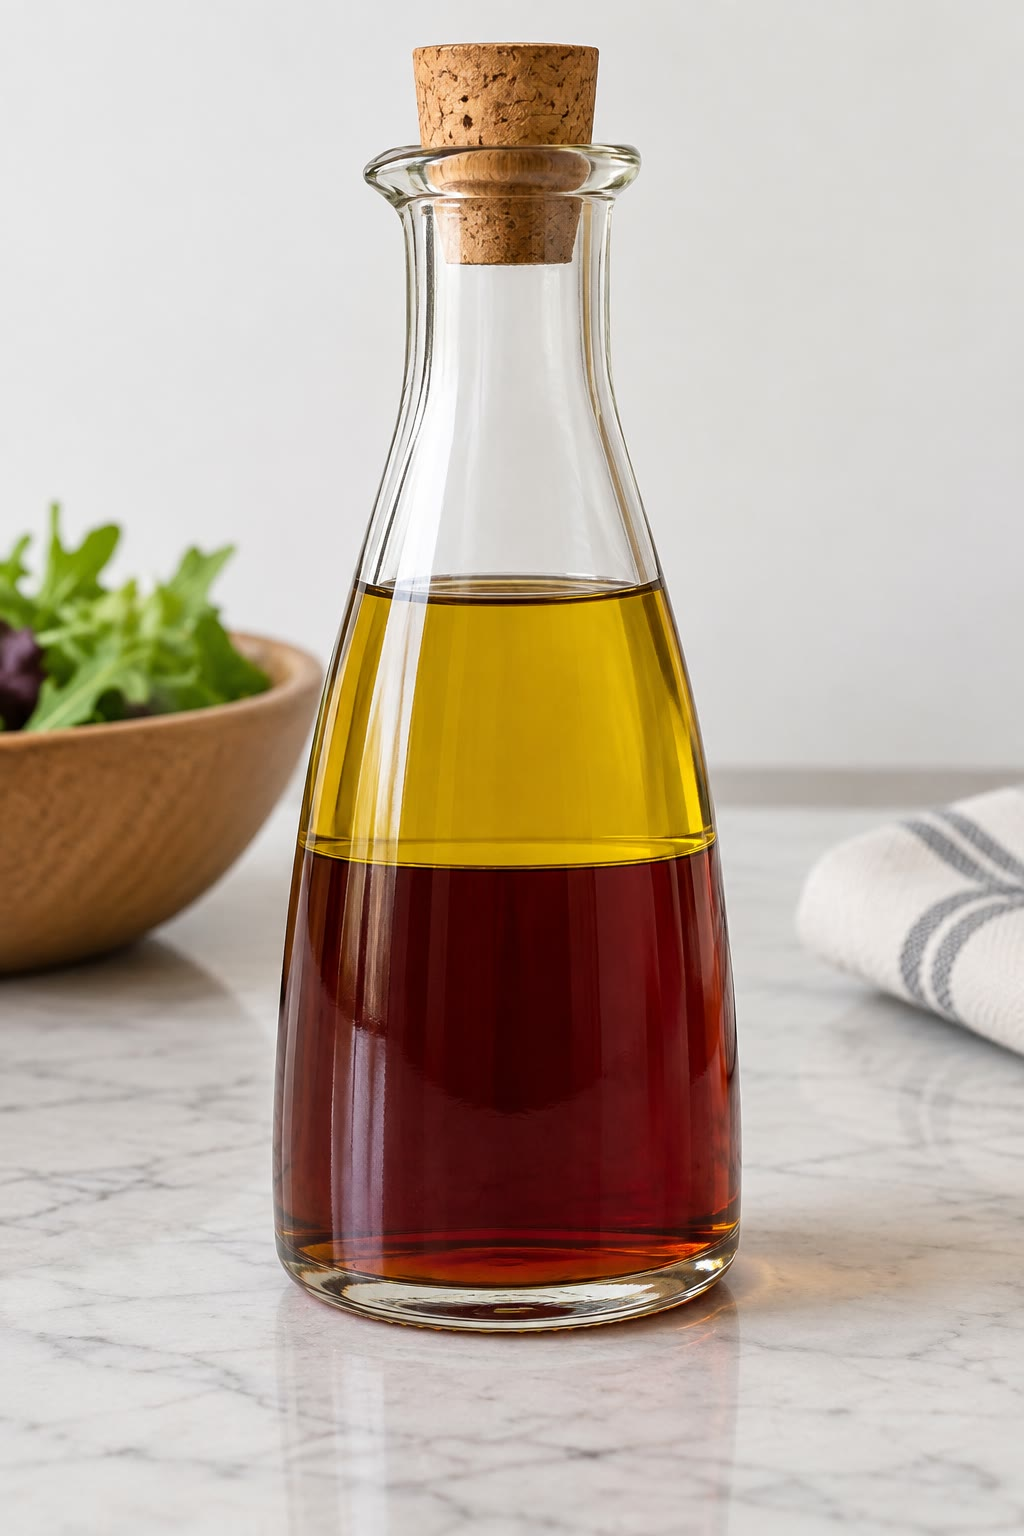
\includegraphics[width=0.2\linewidth]{images/book2/ai/b1-04-dressing.jpg}

{\small Une vinaigrette au repos~: l'huile d'olive, apolaire, flotte sur
le vinaigre, une solution aqueuse~; les deux liquides ne sont pas
\omterm{def:b1:intermolecular-forces-solvents:miscibility}{miscibles}.}
\end{omfigure}

\begin{definition}[Hydrophile, hydrophobe, amphiphile]\label{def:b1:intermolecular-forces-solvents:amphiphile}
Un groupe est \emph{hydrophile}\index{hydrophile} lorsqu'il interagit
favorablement avec l'eau (groupes ioniques ou polaires~: \ce{-COO^-},
\ce{-OH}, \ce{-SO3^-}) et \emph{hydrophobe}\index{hydrophobe} dans le
cas contraire (chaînes hydrocarbonées). Une molécule est
\emph{amphiphile}\index{amphiphile} lorsqu'elle porte à la fois une
tête hydrophile et une queue hydrophobe.
\end{definition}

\begin{example}[Le savon]\label{ex:b1:intermolecular-forces-solvents:soap}
Le dodécanoate de sodium, \ce{CH3(CH2)10COO- Na+}, est \omterm{def:b1:intermolecular-forces-solvents:amphiphile}{amphiphile}. À la
surface de l'eau, ses molécules se dressent, la tête dans l'eau et la
queue dans l'air. Au sein du liquide, au-delà d'une faible concentration,
elles se rassemblent en sphères --- les micelles --- les queues à
l'intérieur et les têtes à l'extérieur. La graisse, apolaire, se dissout
dans le cœur \omterm{def:b1:intermolecular-forces-solvents:amphiphile}{hydrophobe} des micelles et est emportée par l'eau.
\end{example}

\begin{omfigure}
\begin{tikzpicture}[font=\small]
  % interface
  \fill[omWater] (-3.2,-1.6) rectangle (-0.4,0);
  \draw[omDef!60] (-3.2,0) -- (-0.4,0);
  \node[anchor=south west] at (-3.2,0.95) {air};
  \node[anchor=north west] at (-3.2,-1.2) {eau};
  \foreach \x in {-2.9,-2.5,...,-0.6} {
    \fill[omThm] (\x,-0.12) circle (0.11);
    \draw[thick, black!70, decorate, decoration={zigzag, amplitude=1pt, segment length=3pt}] (\x,0) -- (\x,0.85);
  }
  % micelle
  \begin{scope}[xshift=3.2cm, yshift=-0.4cm]
    \fill[omWater] (-2,-1.6) rectangle (2,1.6);
    \foreach \a in {0,30,...,330} {
      \draw[thick, black!70, decorate, decoration={zigzag, amplitude=1pt, segment length=3pt}] (\a:0.25) -- (\a:1.0);
      \fill[omThm] (\a:1.12) circle (0.11);
    }
    \node[anchor=north] at (0,-1.65) {une micelle dans l'eau};
  \end{scope}
\end{tikzpicture}

{\small Molécules \omterm{def:b1:intermolecular-forces-solvents:amphiphile}{amphiphiles} (tête \omterm{def:b1:intermolecular-forces-solvents:amphiphile}{hydrophile} rouge, queue \omterm{def:b1:intermolecular-forces-solvents:amphiphile}{hydrophobe} en
zigzag) à la surface de l'eau et rassemblées en une micelle, dessinée en
coupe~; les micelles sont étudiées dans le volume de troisième année.}
\end{omfigure}

\begin{method}[Choisir un solvant]\label{met:b1:intermolecular-forces-solvents:choose}
Pour choisir un solvant pour un soluté ou pour une réaction~:
\begin{enumerate}
  \item caractériser le soluté~: ionique, polaire, capable de donner ou
        d'accepter des \omterm{def:b1:intermolecular-forces-solvents:hbond}{liaisons hydrogène}, ou apolaire~;
  \item choisir un solvant de même nature (\cref{prop:b1:intermolecular-forces-solvents:like}),
        de forte permittivité s'il faut séparer des ions~;
  \item pour une réaction entre un anion et une molécule, préférer un
        \omterm{def:b1:intermolecular-forces-solvents:solvent-classes}{solvant polaire} aprotique, qui dissout le sel sans lier l'anion
        par \omterm{def:b1:intermolecular-forces-solvents:hbond}{liaisons hydrogène} (\cref{ch:b1:nucleophilic-substitution})~;
  \item pour une extraction, choisir un solvant non \omterm{def:b1:intermolecular-forces-solvents:miscibility}{miscible} au premier
        et dans lequel le soluté est beaucoup plus soluble.
\end{enumerate}
\end{method}

\section{Exercices}

\begin{exercise}[$\star$]\label{exo:b1:intermolecular-forces-solvents:1}
Nommer les interactions présentes entre les particules de l'argon
liquide, du chlorure d'hydrogène liquide, de l'eau liquide, du méthane
liquide et du diiode solide, et dire laquelle domine dans chaque cas.
\end{exercise}

\begin{exercise}[$\star$]\label{exo:b1:intermolecular-forces-solvents:2}
Lesquelles de ces substances forment des \omterm{def:b1:intermolecular-forces-solvents:hbond}{liaisons hydrogène} entre leurs
propres molécules~: \ce{CH3OH}, \ce{CH3OCH3}, \ce{CH3NH2}, \ce{CH3F},
\ce{HF}, \ce{CH4}~? Lesquelles peuvent seulement accepter des \omterm{def:b1:intermolecular-forces-solvents:hbond}{liaisons
hydrogène} d'une autre molécule~?
\end{exercise}

\begin{exercise}[$\star$]\label{exo:b1:intermolecular-forces-solvents:3}
À l'aide du tableau des solvants, classer l'eau, l'éthanol, la propanone,
l'hexane, le dichlorométhane et l'acétonitrile en polaires ou apolaires,
protiques ou aprotiques.
\end{exercise}

\begin{exercise}[$\star$]\label{exo:b1:intermolecular-forces-solvents:4}
Expliquer pourquoi le diiode se dissout beaucoup mieux dans l'hexane que
dans l'eau, et pourquoi le chlorure de sodium fait l'inverse.
\end{exercise}

\begin{exercise}[$\star\star$]\label{exo:b1:intermolecular-forces-solvents:5}
Le méthanol bout à \qty{64.7}{\celsius}, l'éthanol à \qty{78.4}{\celsius},
l'acide éthanoïque à \qty{118.1}{\celsius} et le méthoxyméthane à
\qty{-25.0}{\celsius}. Expliquer cet ordre.
% ledger: bp:CH3OH, bp:C2H5OH, bp:CH3COOH, bp:CH3OCH3
\end{exercise}

\begin{exercise}[$\star\star$]\label{exo:b1:intermolecular-forces-solvents:6}
Calculer la force de Coulomb entre un ion \ce{Na+} et un ion \ce{Cl-}
distants de \qty{500}{pm} dans le vide ($\varepsilon_0 = \qty{8.854e-12}{F/m}$,
$e = \qty{1.602e-19}{C}$), puis dans l'eau ($\varepsilon_r = 78.4$) et
dans l'hexane ($\varepsilon_r = 1.89$). Commenter.
\end{exercise}

\begin{exercise}[$\star\star$]\label{exo:b1:intermolecular-forces-solvents:7}
La propanone et l'eau sont \omterm{def:b1:intermolecular-forces-solvents:miscibility}{miscibles} en toutes proportions~; l'hexane et
l'eau ne le sont pas. Expliquer, en considérant les interactions rompues
et formées.
\end{exercise}

\begin{exercise}[$\star\star$]\label{exo:b1:intermolecular-forces-solvents:8}
\ce{HCl} a un \omterm{def:b1:lewis-resonance-vsepr:dipole}{moment dipolaire} de \qty{1.09}{\debye} et bout à
\qty{-85.0}{\celsius}~; \ce{HBr} a \qty{0.83}{\debye} et bout à
\qty{-66.4}{\celsius}. Pourquoi la molécule la moins polaire bout-elle
plus haut~?
% ledger: dip:HCl, dip:HBr, bp:HCl, bp:HBr
\end{exercise}

\begin{exercise}[$\star\star$]\label{exo:b1:intermolecular-forces-solvents:9}
Dessiner le dimère cyclique de l'acide éthanoïque. En solution dans le
benzène, l'acide éthanoïque se comporte comme si sa masse molaire valait
environ deux fois \qty{60}{g/mol}~; dans l'eau, non. Expliquer ces deux
faits.
\end{exercise}

\begin{exercise}[$\star\star\star$]\label{exo:b1:intermolecular-forces-solvents:10}
Décrire la dissolution du chlorure de sodium dans l'eau en termes de
dissociation et de \omterm{def:b1:intermolecular-forces-solvents:dissolution}{solvatation}, et celle du chlorure d'hydrogène dans
l'eau en termes d'ionisation, de dissociation et de \omterm{def:b1:intermolecular-forces-solvents:dissolution}{solvatation}. Pourquoi
le chlorure d'hydrogène dans l'hexane donne-t-il une solution non
conductrice~?
\end{exercise}

\begin{exercise}[$\star\star\star$]\label{exo:b1:intermolecular-forces-solvents:11}
À partir des températures d'ébullition des alcanes linéaires (pentane
\qty{36.1}{\celsius}, décane \qty{174.1}{\celsius}), calculer
l'augmentation moyenne par groupe \ce{CH2} entre \ce{C5} et \ce{C10}, et
estimer la température d'ébullition de l'undécane. Pourquoi l'incrément
diminue-t-il le long de la série~?
% ledger: bp:C5H12, bp:C10H22
\end{exercise}

\begin{exercise}[$\star\star\star$]\label{exo:b1:intermolecular-forces-solvents:12}
Le dodécylsulfate de sodium, \ce{CH3(CH2)11OSO3^- Na+}, est un
détergent. Identifier ses parties \omterm{def:b1:intermolecular-forces-solvents:amphiphile}{hydrophile} et \omterm{def:b1:intermolecular-forces-solvents:amphiphile}{hydrophobe}, schématiser
son organisation à la surface de l'eau et dans une micelle, et expliquer
comment il élimine une tache grasse d'un tissu.
\end{exercise}

\section{Problème~: si l'eau n'avait pas de liaisons hydrogène}

\begin{problem}[{Problème du week-end --- les forces de London dans les
gaz nobles et les alcanes, le choix d'un solvant, et la température
d'ébullition qu'aurait l'eau sans liaisons hydrogène}]
\label{pb:b1:intermolecular-forces-solvents:1}
Températures d'ébullition sous \qty{1}{atm} (en \unit{\celsius})~:
\ce{He} $-268.9$,
\ce{Ne} $-246.1$, \ce{Ar} $-185.9$, \ce{Kr} $-153.4$, \ce{Xe} $-108.1$~;
pentane 36.1, hexane 68.8~; \ce{CH4} $-161.5$, \ce{SiH4} $-112.0$,
\ce{GeH4} $-88.1$~; \ce{NH3} $-33.4$, \ce{PH3} $-87.8$, \ce{AsH3} $-62.5$~;
\ce{H2O} 100.0, \ce{H2S} $-60.3$, \ce{H2Se} $-41.3$~; \ce{HF} 19.6,
\ce{HCl} $-85.0$, \ce{HBr} $-66.4$.
% ledger: bp:He, bp:Ne, bp:Ar, bp:Kr, bp:Xe, bp:C5H12, bp:C6H14, bp:CH4,
% bp:SiH4, bp:GeH4, bp:NH3, bp:PH3, bp:AsH3, bp:H2O, bp:H2S, bp:H2Se,
% bp:HF, bp:HCl, bp:HBr

\medskip
\noindent\textbf{Partie I --- London seul.}
\begin{enumerate}
  \item Quelle interaction assure la cohésion des atomes de l'argon
        liquide~?
  \item Expliquer l'augmentation de la température d'ébullition de
        l'hélium au xénon.
  \item Pourquoi la température d'ébullition de l'hélium est-elle la plus
        basse de toutes les substances~?
  \item Comparer le pentane et l'hexane~: qu'apporte un groupe \ce{CH2}~?
  \item Le méthane, le silane et le germane n'ont pas de \omterm{def:b1:lewis-resonance-vsepr:dipole}{moment
        dipolaire}. Quelle interaction explique l'ordre de leurs
        températures d'ébullition~?
  \item Pourquoi aucune \omterm{def:b1:intermolecular-forces-solvents:hbond}{liaison hydrogène} n'est-elle possible dans le
        méthane~?
\end{enumerate}

\medskip
\noindent\textbf{Partie II --- Choisir des solvants.}
Utiliser le tableau des solvants du chapitre.
\begin{enumerate}[resume]
  \item Quel solvant du tableau dissout le mieux le chlorure de sodium,
        et pourquoi~?
  \item De quel facteur l'attraction entre deux ions est-elle plus faible
        dans l'eau que dans l'hexane, à la même distance~?
  \item Une réaction entre l'anion \ce{CN-} et une molécule organique
        doit être menée dans un solvant qui dissout le sel sans lier
        l'anion par \omterm{def:b1:intermolecular-forces-solvents:hbond}{liaisons hydrogène}. En choisir un.
  \item Pour extraire le diiode d'une solution aqueuse, quel solvant du
        tableau choisir, et dans quelle phase le diiode se
        retrouvera-t-il~?
  \item Expliquer pourquoi l'éthanol ne convient pas à cette extraction.
  \item L'éthoxyéthane est à peine \omterm{def:b1:intermolecular-forces-solvents:miscibility}{miscible} à l'eau bien qu'il soit
        polaire. Proposer une explication.
\end{enumerate}

\medskip
\noindent\textbf{Partie III --- Les autres hydrures.}
\begin{enumerate}[resume]
  \item Pour le \omterm{def:b1:periodicity:table}{groupe} 17, calculer la variation de la température
        d'ébullition de \ce{HCl} à \ce{HBr}, et extrapoler la même
        variation jusqu'à la \omterm{def:b1:periodicity:table}{période} 2.
  \item Comparer la valeur extrapolée à la température d'ébullition de
        \ce{HF}.
  \item Mêmes deux questions pour le \omterm{def:b1:periodicity:table}{groupe} 15 (\ce{PH3}, \ce{AsH3} et
        \ce{NH3}).
  \item Pour le \omterm{def:b1:periodicity:table}{groupe} 14, \ce{CH4} est-il au-dessus ou au-dessous de
        l'extrapolation à partir de \ce{SiH4} et \ce{GeH4}~? Pourquoi
        n'est-ce pas surprenant~?
  \item Classer les excédents de \ce{NH3}, de \ce{HF} et de l'eau.
  \item Compter les \omterm{def:b1:intermolecular-forces-solvents:hbond}{liaisons hydrogène} que chaque molécule de \ce{NH3},
        de \ce{HF} et de \ce{H2O} peut donner et accepter, et expliquer
        le classement.
\end{enumerate}

\medskip
\noindent\textbf{Partie IV --- L'eau sans \omterm{def:b1:intermolecular-forces-solvents:hbond}{liaisons hydrogène}.}
\begin{enumerate}[resume]
  \item Pourquoi \ce{H2S} et \ce{H2Se} conviennent-ils à une
        extrapolation, et pourquoi pas l'eau elle-même~?
  \item Calculer la variation de la température d'ébullition de \ce{H2S}
        à \ce{H2Se}.
  \item Écrire l'équation de la droite passant par ces deux points, avec
        la \omterm{def:b1:periodicity:table}{période} $p$ pour variable.
  \item En déduire la température d'ébullition qu'aurait l'eau pour
        $p = 2$.
  \item De combien les \omterm{def:b1:intermolecular-forces-solvents:hbond}{liaisons hydrogène} élèvent-elles la température
        d'ébullition de l'eau~?
  \item Conclure~: à quelle température l'eau bouillirait-elle si ses
        molécules s'attiraient comme celles de \ce{H2S}~?
\end{enumerate}
\end{problem}
